\documentclass[11pt]{article}
\usepackage{epsf,amsmath,amsfonts,amsthm,graphicx,color}
%\usepackage{draftcopy}
\textwidth=7in
\textheight=11.0in
\hoffset=-1in
\voffset=-1in
\bibliographystyle{alpha}


\usepackage{amsthm, amsmath, amssymb, amsfonts, graphicx, graphics,epsfig, bbm, xcolor, hyperref,subfigure,float}


\newcommand{\xinnote}[1]{ {\textcolor{red}  {\mbox{**Xin:} #1}}}
\newcommand{\nichollsnote}[1]{ {\textcolor{yellow}  {\mbox{**Nicholls:} #1}}}
\newcommand{\hpra}{\frac{H_p^{(1)}(kr)}{H_p^{(1)}(ka)} }
\newcommand{\hprb}{\frac{H_p^{(1)}(kr)}{H_p^{(1)}(kb)} }
\newcommand{\diffhpn}{\frac{d_z^nH_p^{(1)}(ka)}{H_p^{(1)}(ka)} }
\newcommand{\diffhpnm}{\frac{d_z^{n-m}H_p^{(1)}(ka)}{H_p^{(1)}(ka)} }
\newcommand{\ep}{e^{ip\theta}}
\newcommand{\opD}{\mathcal{D}}
\newcommand{\jpra}{\frac{J_p(kr)}{J_p(ka)} }
\newcommand{\diffjpn}{\frac{d_z^nJ_p(ka)}{J_p(ka)} }
\newcommand{\diffjpnm}{\frac{d_z^{n-m}J_p(ka)}{J_p(ka)} }

\renewcommand*{\thesubfigure}{(\thefigure.\arabic{subfigure})}

\begin{document}
\noindent\textbf{\large IIO FE---Numerical results}\\
\section{$\exp(\cos \theta)$}
\noindent\textbf{$f(x)=\exp(\cos \theta) $, Eps\_max = 0.1*a =0.0025, outer = VACUUM, inner = SILVER }\\
	a = 0.025, b = 0.25, N\_theta = 64, N = 16, M = 201,  N\_eps = 201
	
\begin{figure}[H]
	\centering
	\subfigure [IIO (Qu) ] 
	{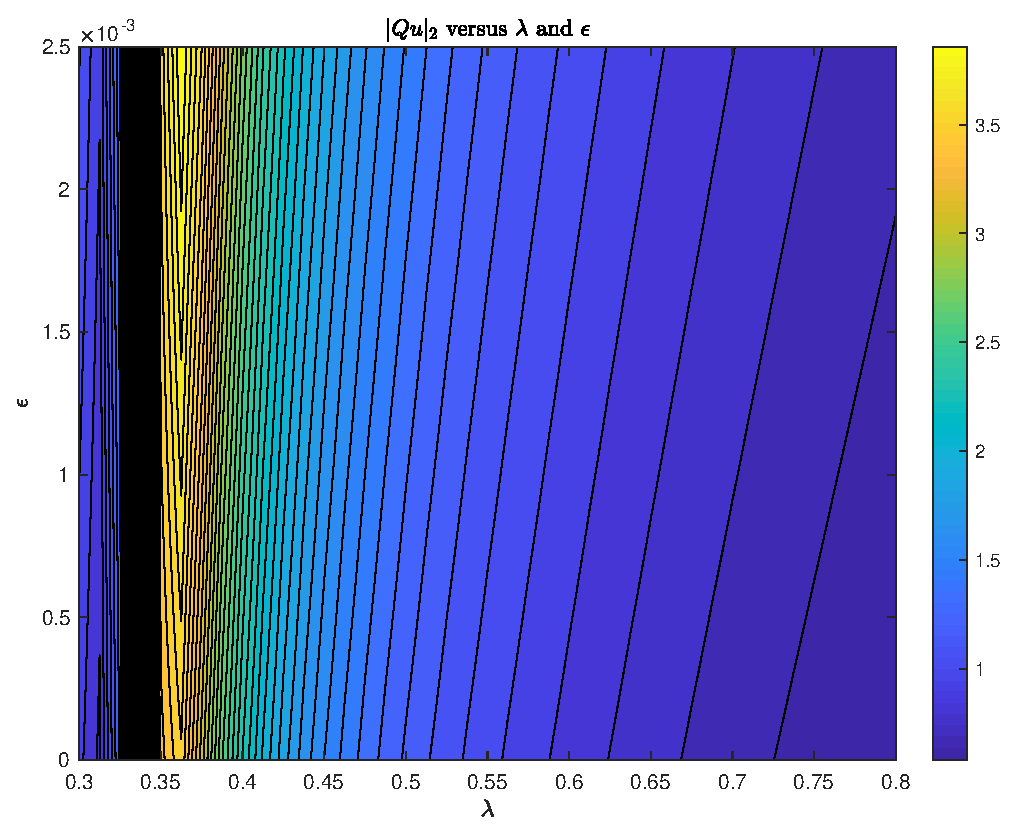
\includegraphics[width=0.35\textwidth]
		{fig_IIO_Qu_expcos_eps10lamSILVERVACUUM.pdf}}
	\quad
	\subfigure [IIO (Sw)] 
	{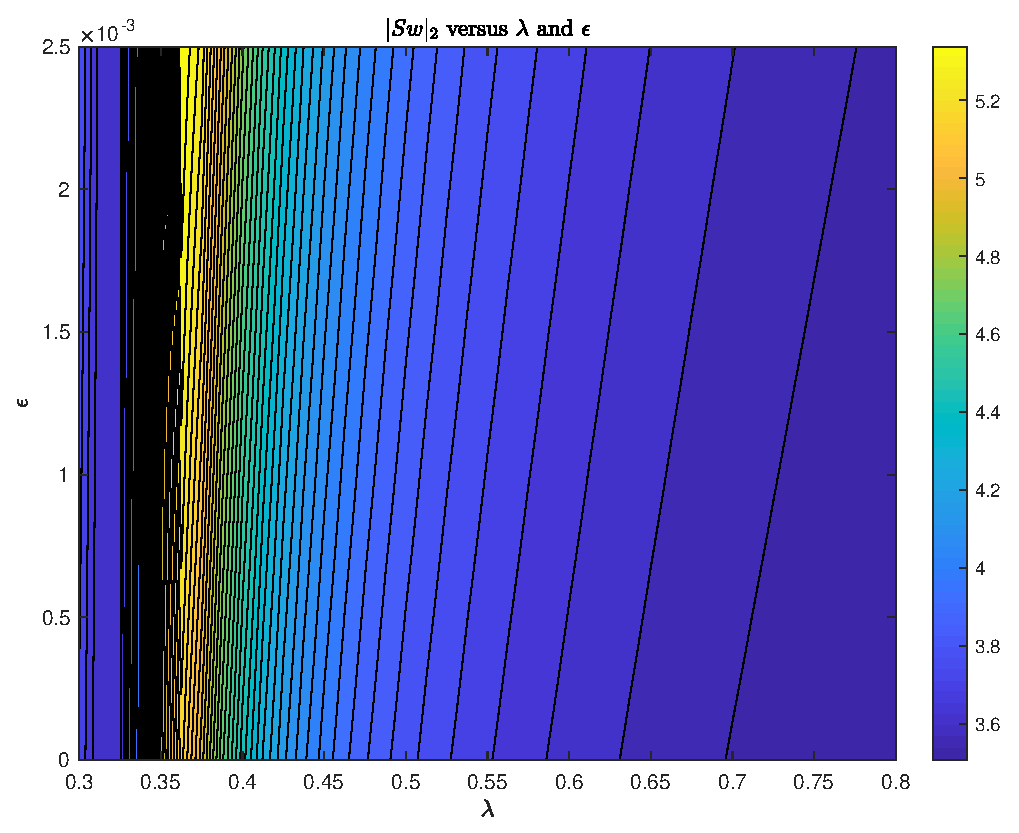
\includegraphics[width=0.35\textwidth]
		{fig_IIO_Sw_expcos_eps10lamSILVERVACUUM.pdf}}
	\\
	\subfigure [BU ratio] 
	{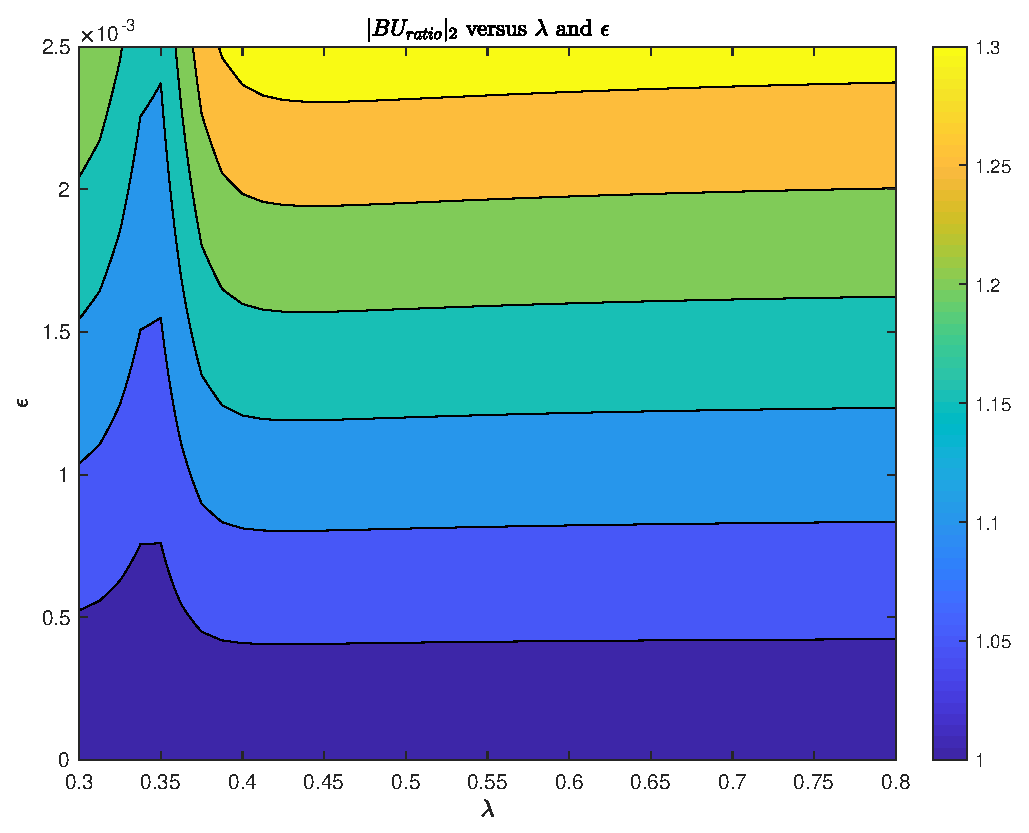
\includegraphics[width=0.35\textwidth]
		{fig_IIO_BU_expcos_eps10lamSILVERVACUUM.pdf}}
	\quad
	\subfigure [BU ratio] 
	{\includegraphics[width=0.35\textwidth]
		{fig_IIO_BUratiolam_expcos_eps10SILVERVACUUM.pdf}}	
	\\
	\subfigure [$\tilde{U}$ and $\tilde{W}$] 
	{\includegraphics[width=0.35\textwidth]
		{fig_IIO_UWlam_expcos_eps10SILVERVACUUM.pdf}}
	\quad
	\subfigure [Qu and Sw] 
	{\includegraphics[width=0.35\textwidth]
		{fig_IIO_QuSwlam_expcos_eps10SILVERVACUUM.pdf}}
	\caption{$\exp(\cos \theta)$ with Eps\_max = 0.1*a}
\end{figure}

\newpage
\noindent\textbf{$f(x)=\exp(\cos \theta) $, Eps\_max = 0.2*a =0.0025, outer = VACUUM, inner = SILVER }\\
a = 0.025, b = 0.25, N\_theta = 64, N = 16, M = 201,  N\_eps = 201

\begin{figure}[H]
	\centering
	\subfigure [IIO (Qu) ] 
	{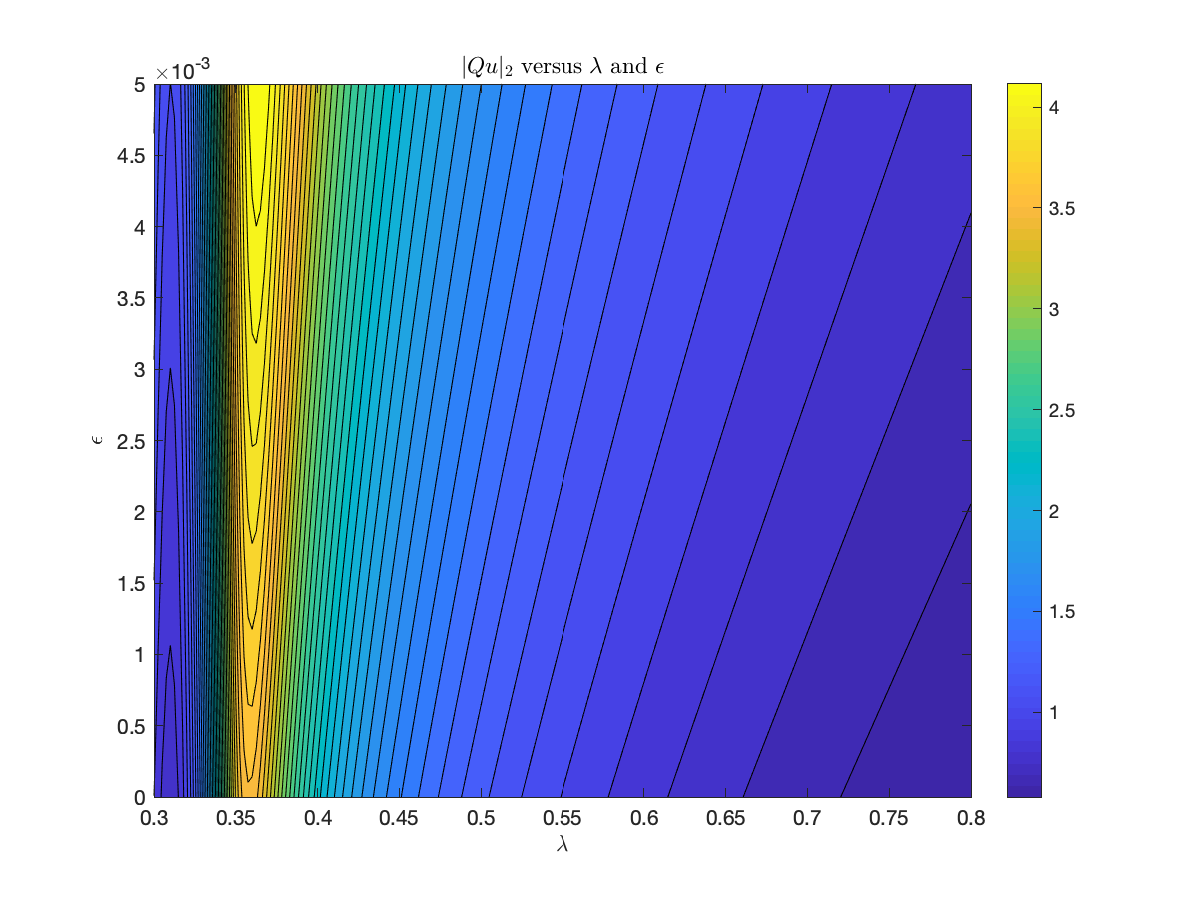
\includegraphics[width=0.35\textwidth]
		{fig_IIO_Qu_expcos_eps20lamSILVERVACUUM.pdf}}
	\quad
	\subfigure [IIO (Sw)] 
	{\includegraphics[width=0.35\textwidth]
		{fig_IIO_Sw_expcos_eps20lamSILVERVACUUM.pdf}}
	\\
	\subfigure [BU ratio] 
	{\includegraphics[width=0.35\textwidth]
		{fig_IIO_BU_expcos_eps20lamSILVERVACUUM.pdf}}
	\quad
	\subfigure [BU ratio] 
	{\includegraphics[width=0.35\textwidth]
		{fig_IIO_BUratiolam_expcos_eps20SILVERVACUUM.pdf}}
	\subfigure [$\tilde{U}$ and $\tilde{W}$] 
	{\includegraphics[width=0.35\textwidth]
		{fig_IIO_UWlam_expcos_eps20SILVERVACUUM.pdf}}
	\quad
	\subfigure [Qu and Sw] 
	{\includegraphics[width=0.35\textwidth]
		{fig_IIO_QuSwlam_expcos_eps20SILVERVACUUM.pdf}}
	\caption{$\exp(\cos \theta)$ with Eps\_max = 0.2*a}
\end{figure}

\newpage
\noindent\textbf{$f(x)=\exp(\cos \theta) $, Eps\_max = 0.1*a =0.0025, outer = WATER, inner = SILVER }\\
a = 0.025, b = 0.25, N\_theta = 64, N = 16, M = 201,  N\_eps = 201

\begin{figure}[H]
	\centering
	\subfigure [IIO (Qu) ] 
	{\includegraphics[width=0.35\textwidth]
		{fig_IIO_Qu_expcos_eps10lamSILVERWATER.pdf}}
	\quad
	\subfigure [IIO (Sw)] 
	{\includegraphics[width=0.35\textwidth]
		{fig_IIO_Sw_expcos_eps10lamSILVERWATER.pdf}}
	\\
	\subfigure [BU ratio] 
	{\includegraphics[width=0.35\textwidth]
		{fig_IIO_BU_expcos_eps10lamSILVERWATER.pdf}}
	\quad
	\subfigure [BU ratio] 
	{\includegraphics[width=0.35\textwidth]
		{fig_IIO_BUratiolam_expcos_eps10SILVERWATER.pdf}}
	\\	
	\subfigure [$\tilde{U}$ and $\tilde{W}$] 
	{\includegraphics[width=0.35\textwidth]
		{fig_IIO_UWlam_expcos_eps10SILVERWATER.pdf}}
	\quad
	\subfigure [Qu and Sw] 
	{\includegraphics[width=0.35\textwidth]
		{fig_IIO_QuSwlam_expcos_eps10SILVERWATER.pdf}}
	\caption{$\exp(\cos \theta)$ with Eps\_max = 0.1*a}
\end{figure}

\newpage
\noindent\textbf{$f(x)=\exp(\cos \theta) $, Eps\_max = 0.2*a =0.0025, outer = WATER, inner = SILVER }\\
a = 0.025, b = 0.25, N\_theta = 64, N = 16, M = 201,  N\_eps = 201

\begin{figure}[H]
	\centering
	\subfigure [IIO (Qu) ] 
	{\includegraphics[width=0.35\textwidth]
		{fig_IIO_Qu_expcos_eps20lamSILVERWATER.pdf}}
	\quad
	\subfigure [IIO (Sw)] 
	{\includegraphics[width=0.35\textwidth]
		{fig_IIO_Sw_expcos_eps20lamSILVERWATER.pdf}}
	\\
	\subfigure [BU ratio] 
	{\includegraphics[width=0.35\textwidth]
		{fig_IIO_BU_expcos_eps20lamSILVERWATER.pdf}}
	\quad
	\subfigure [BU ratio] 
	{\includegraphics[width=0.35\textwidth]
		{fig_IIO_BUratiolam_expcos_eps20SILVERWATER.pdf}}
	\\
	\subfigure [$\tilde{U}$ and $\tilde{W}$] 
	{\includegraphics[width=0.35\textwidth]
		{fig_IIO_UWlam_expcos_eps20SILVERWATER.pdf}}
	\quad
	\subfigure [Qu and Sw] 
	{\includegraphics[width=0.35\textwidth]
		{fig_IIO_QuSwlam_expcos_eps20SILVERWATER.pdf}}
	\caption{$\exp(\cos \theta)$ with Eps\_max = 0.2*a}
\end{figure}

\newpage
\section{$\cos 2\theta$ }
\noindent\textbf{$f(x) = \cos 2 \theta $, Eps\_max = 0.1*a =0.0025, outer = VACUUM, inner = SILVER }\\
a = 0.025, b = 0.25, N\_theta = 64, N = 16, M = 201,  N\_eps = 201

\begin{figure}[H]
	\centering
	\subfigure [IIO (Qu) ] 
	{\includegraphics[width=0.35\textwidth]
		{fig_IIO_Qu_cos2_eps10lamSILVERVACUUM.pdf}}
	\quad
	\subfigure [IIO (Sw)] 
	{\includegraphics[width=0.35\textwidth]
		{fig_IIO_Sw_cos2_eps10lamSILVERVACUUM.pdf}}
	\\
	\subfigure [BU ratio] 
	{\includegraphics[width=0.35\textwidth]
		{fig_IIO_BU_cos2_eps10lamSILVERVACUUM.pdf}}
	\quad
	\subfigure [BU ratio] 
	{\includegraphics[width=0.35\textwidth]
		{fig_IIO_BUratiolam_cos2_eps10SILVERVACUUM.pdf}}	
	\\
	\subfigure [$\tilde{U}$ and $\tilde{W}$] 
	{\includegraphics[width=0.35\textwidth]
		{fig_IIO_UWlam_cos2_eps10SILVERVACUUM.pdf}}
	\quad
	\subfigure [Qu and Sw] 
	{\includegraphics[width=0.35\textwidth]
		{fig_IIO_QuSwlam_cos2_eps10SILVERVACUUM.pdf}}
	\caption{$\cos 2\theta$ with Eps\_max = 0.1*a}
\end{figure}

\newpage
\noindent\textbf{$f(x)= \cos 2 \theta $, Eps\_max = 0.2*a =0.0025, outer = VACUUM, inner = SILVER }\\
a = 0.025, b = 0.25, N\_theta = 64, N = 16, M = 201,  N\_eps = 201

\begin{figure}[H]
	\centering
	\subfigure [IIO (Qu) ] 
	{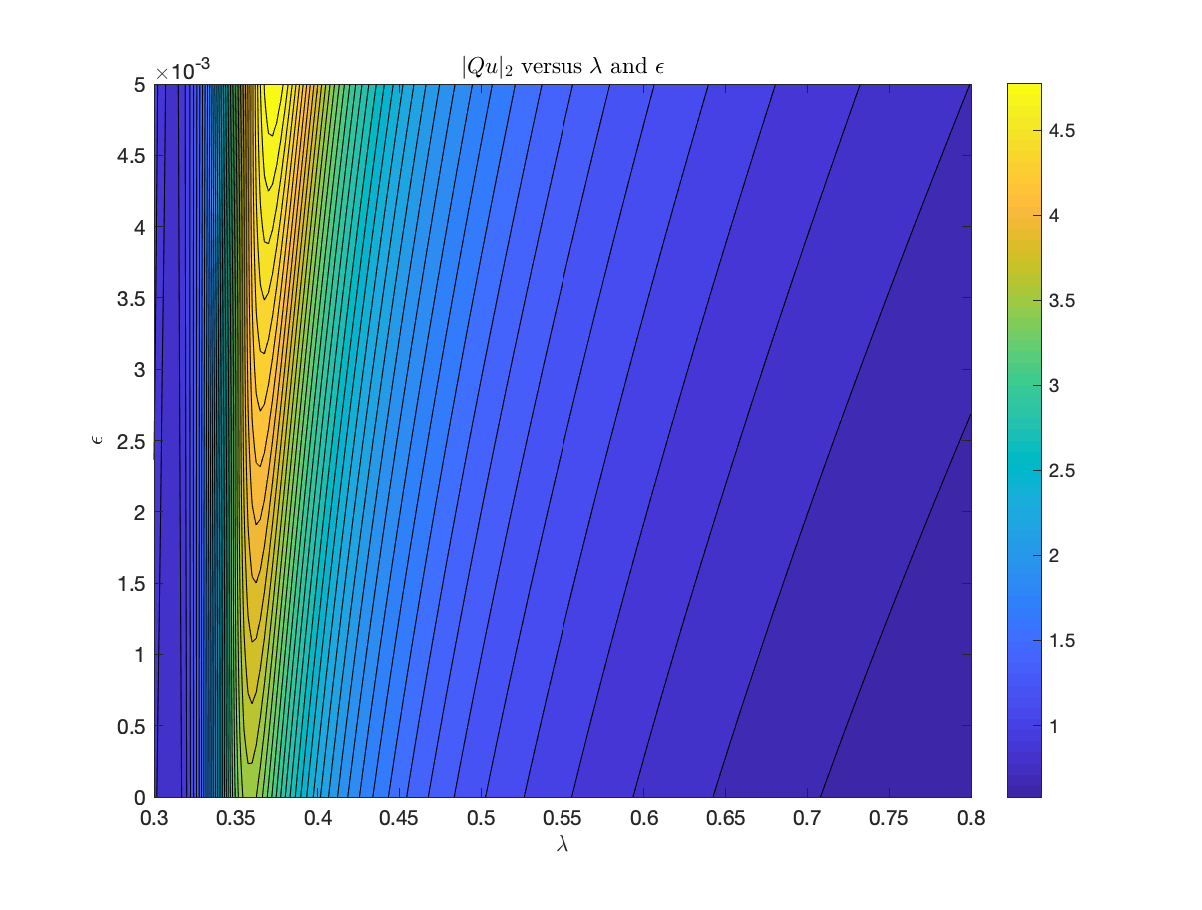
\includegraphics[width=0.35\textwidth]
		{fig_IIO_Qu_cos2_eps20lamSILVERVACUUM.pdf}}
	\quad
	\subfigure [IIO (Sw)] 
	{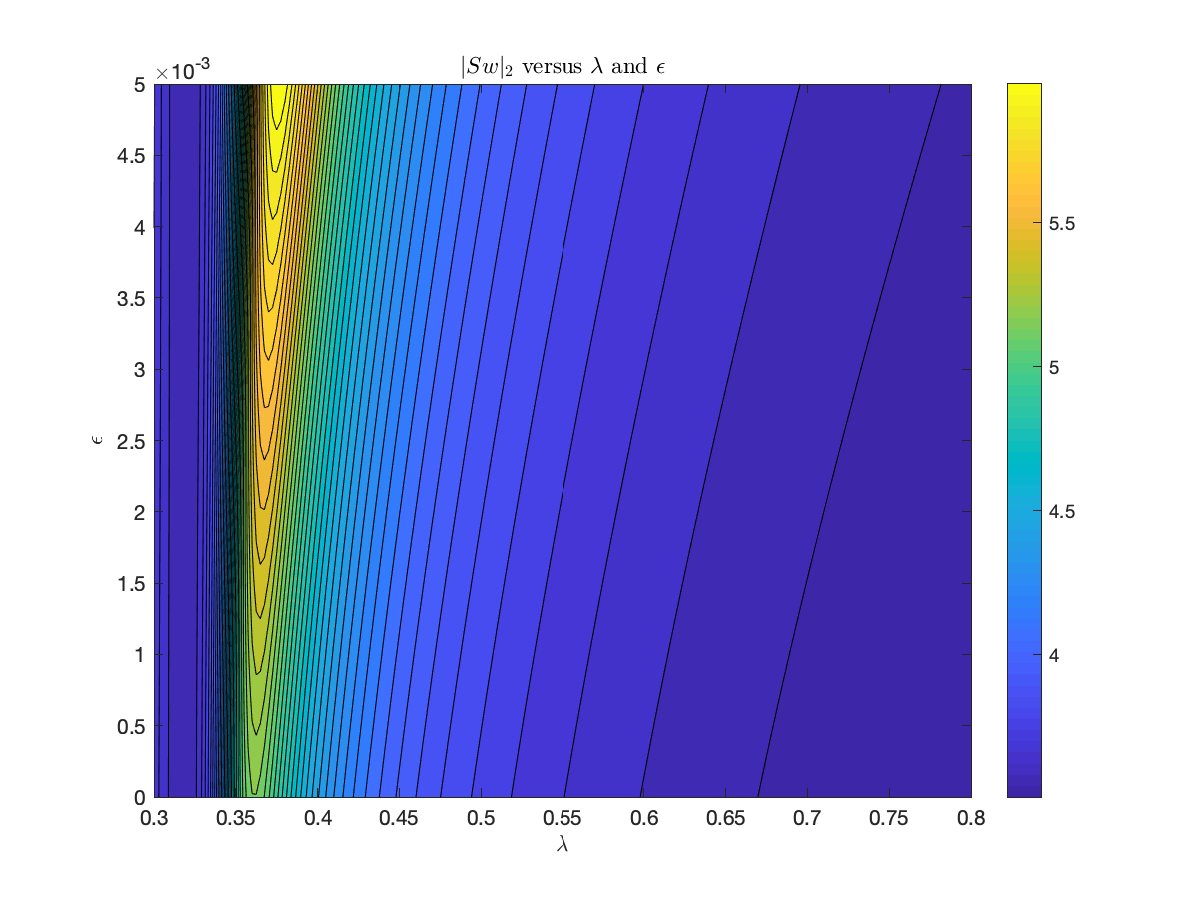
\includegraphics[width=0.35\textwidth]
		{fig_IIO_Sw_cos2_eps20lamSILVERVACUUM.pdf}}
	\\
	\subfigure [BU ratio] 
	{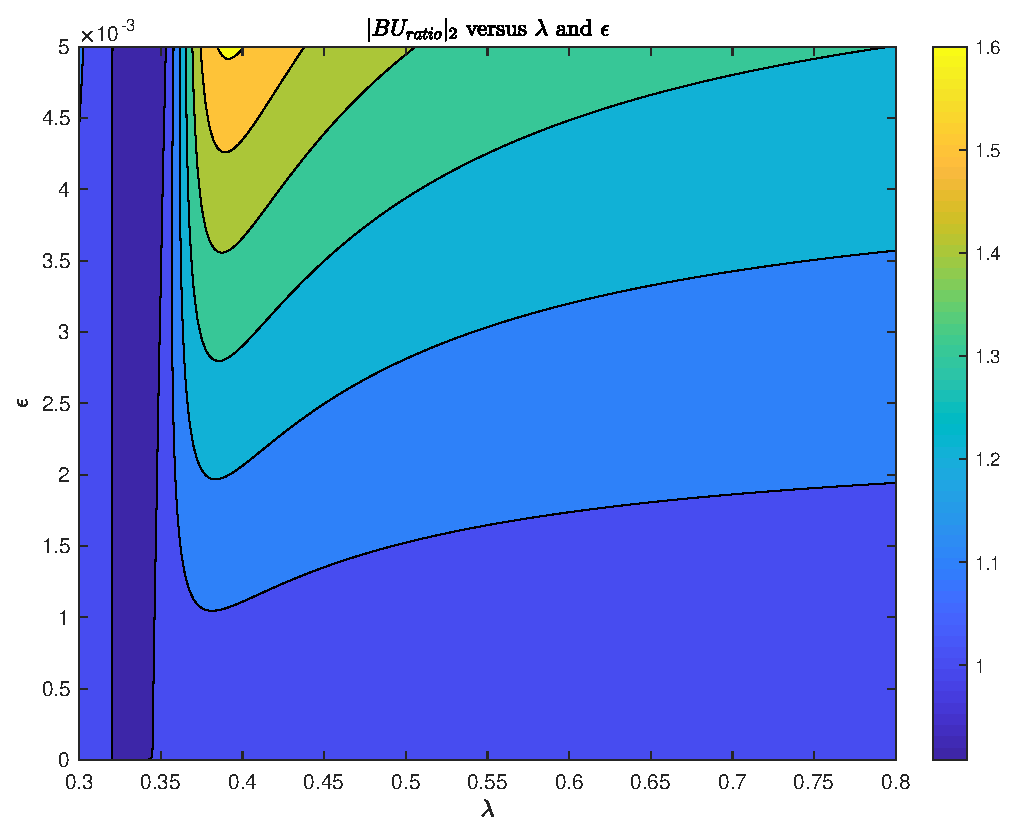
\includegraphics[width=0.35\textwidth]
		{fig_IIO_BU_cos2_eps20lamSILVERVACUUM.pdf}}
	\quad
	\subfigure [BU ratio] 
	{\includegraphics[width=0.35\textwidth]
		{fig_IIO_BUratiolam_cos2_eps20SILVERVACUUM.pdf}}
	\subfigure [$\tilde{U}$ and $\tilde{W}$] 
	{\includegraphics[width=0.35\textwidth]
		{fig_IIO_UWlam_cos2_eps20SILVERVACUUM.pdf}}
	\quad
	\subfigure [Qu and Sw] 
	{\includegraphics[width=0.35\textwidth]
		{fig_IIO_QuSwlam_cos2_eps20SILVERVACUUM.pdf}}
	\caption{$\cos 2\theta$ with Eps\_max = 0.2*a}
\end{figure}

\newpage
\noindent\textbf{$f(x)= \cos 2 \theta $, Eps\_max = 0.1*a =0.0025, outer = WATER, inner = SILVER }\\
a = 0.025, b = 0.25, N\_theta = 64, N = 16, M = 201,  N\_eps = 201

\begin{figure}[H]
	\centering
	\subfigure [IIO (Qu) ] 
	{\includegraphics[width=0.35\textwidth]
		{fig_IIO_Qu_cos2_eps10lamSILVERWATER.pdf}}
	\quad
	\subfigure [IIO (Sw)] 
	{\includegraphics[width=0.35\textwidth]
		{fig_IIO_Sw_cos2_eps10lamSILVERWATER.pdf}}
	\\
	\subfigure [BU ratio] 
	{\includegraphics[width=0.35\textwidth]
		{fig_IIO_BU_cos2_eps10lamSILVERWATER.pdf}}
	\quad
	\subfigure [BU ratio] 
	{\includegraphics[width=0.35\textwidth]
		{fig_IIO_BUratiolam_cos2_eps10SILVERWATER.pdf}}
	\\	
	\subfigure [$\tilde{U}$ and $\tilde{W}$] 
	{\includegraphics[width=0.35\textwidth]
		{fig_IIO_UWlam_cos2_eps10SILVERWATER.pdf}}
	\quad
	\subfigure [Qu and Sw] 
	{\includegraphics[width=0.35\textwidth]
		{fig_IIO_QuSwlam_cos2_eps10SILVERWATER.pdf}}
	\caption{$\cos 2\theta$ with Eps\_max = 0.1*a}
\end{figure}

\newpage
\noindent\textbf{$f(x)= \cos 2 \theta $, Eps\_max = 0.2*a =0.0025, outer = WATER, inner = SILVER }\\
a = 0.025, b = 0.25, N\_theta = 64, N = 16, M = 201,  N\_eps = 201

\begin{figure}[H]
	\centering
	\subfigure [IIO (Qu) ] 
	{\includegraphics[width=0.35\textwidth]
		{fig_IIO_Qu_cos2_eps20lamSILVERWATER.pdf}}
	\quad
	\subfigure [IIO (Sw)] 
	{\includegraphics[width=0.35\textwidth]
		{fig_IIO_Sw_cos2_eps20lamSILVERWATER.pdf}}
	\\
	\subfigure [BU ratio] 
	{\includegraphics[width=0.35\textwidth]
		{fig_IIO_BU_cos2_eps20lamSILVERWATER.pdf}}
	\quad
	\subfigure [BU ratio] 
	{\includegraphics[width=0.35\textwidth]
		{fig_IIO_BUratiolam_cos2_eps20SILVERWATER.pdf}}
	\\
	\subfigure [$\tilde{U}$ and $\tilde{W}$] 
	{\includegraphics[width=0.35\textwidth]
		{fig_IIO_UWlam_cos2_eps20SILVERWATER.pdf}}
	\quad
	\subfigure [Qu and Sw] 
	{\includegraphics[width=0.35\textwidth]
		{fig_IIO_QuSwlam_cos2_eps20SILVERWATER.pdf}}
	\caption{$\cos 2\theta$ with Eps\_max = 0.2*a}
\end{figure}

\newpage
\section{$\cos 4\theta$ }
\noindent\textbf{$f(x) = \cos 4 \theta $, Eps\_max = 0.1*a =0.0025, outer = VACUUM, inner = SILVER }\\
a = 0.025, b = 0.25, N\_theta = 64, N = 16, M = 201,  N\_eps = 201

\begin{figure}[H]
	\centering
	\subfigure [IIO (Qu) ] 
	{\includegraphics[width=0.35\textwidth]
		{fig_IIO_Qu_cos4_eps10lamSILVERVACUUM.pdf}}
	\quad
	\subfigure [IIO (Sw)] 
	{\includegraphics[width=0.35\textwidth]
		{fig_IIO_Sw_cos4_eps10lamSILVERVACUUM.pdf}}
	\\
	\subfigure [BU ratio] 
	{\includegraphics[width=0.35\textwidth]
		{fig_IIO_BU_cos4_eps10lamSILVERVACUUM.pdf}}
	\quad
	\subfigure [BU ratio] 
	{\includegraphics[width=0.35\textwidth]
		{fig_IIO_BUratiolam_cos4_eps10SILVERVACUUM.pdf}}	
	\\
	\subfigure [$\tilde{U}$ and $\tilde{W}$] 
	{\includegraphics[width=0.35\textwidth]
		{fig_IIO_UWlam_cos4_eps10SILVERVACUUM.pdf}}
	\quad
	\subfigure [Qu and Sw] 
	{\includegraphics[width=0.35\textwidth]
		{fig_IIO_QuSwlam_cos4_eps10SILVERVACUUM.pdf}}
	\caption{$\cos 2\theta$ with Eps\_max = 0.1*a}
\end{figure}

\newpage
\noindent\textbf{$f(x) = \cos 4 \theta $, Eps\_max = 0.2*a =0.0025, outer = VACUUM, inner = SILVER }\\
a = 0.025, b = 0.25, \textcolor{red}{N\_theta = 128}, N = 16, M = 201,  N\_eps = 201

\begin{figure}[H]
	\centering
	\subfigure [IIO (Qu) ] 
	{\includegraphics[width=0.35\textwidth]
		{fig_IIO_Qu_cos4_eps20lamSILVERVACUUM.pdf}}
	\quad
	\subfigure [IIO (Sw)] 
	{\includegraphics[width=0.35\textwidth]
		{fig_IIO_Sw_cos4_eps20lamSILVERVACUUM.pdf}}
	\\
	\subfigure [BU ratio] 
	{\includegraphics[width=0.35\textwidth]
		{fig_IIO_BU_cos4_eps20lamSILVERVACUUM.pdf}}
	\quad
	\subfigure [BU ratio] 
	{\includegraphics[width=0.35\textwidth]
		{fig_IIO_BUratiolam_cos4_eps20SILVERVACUUM.pdf}}
	\subfigure [$\tilde{U}$ and $\tilde{W}$] 
	{\includegraphics[width=0.35\textwidth]
		{fig_IIO_UWlam_cos4_eps20SILVERVACUUM.pdf}}
	\quad
	\subfigure [Qu and Sw] 
	{\includegraphics[width=0.35\textwidth]
		{fig_IIO_QuSwlam_cos4_eps20SILVERVACUUM.pdf}}
	\caption{$\cos 4\theta$ with Eps\_max = 0.2*a}
\end{figure}

\newpage
\noindent\textbf{$f(x)=\cos 4 \theta $, Eps\_max = 0.1*a =0.0025, outer = WATER, inner = SILVER }\\
a = 0.025, b = 0.25, N\_theta = 64, N = 16, M = 201,  N\_eps = 201

\begin{figure}[H]
	\centering
	\subfigure [IIO (Qu) ] 
	{\includegraphics[width=0.35\textwidth]
		{fig_IIO_Qu_cos4_eps10lamSILVERWATER.pdf}}
	\quad
	\subfigure [IIO (Sw)] 
	{\includegraphics[width=0.35\textwidth]
		{fig_IIO_Sw_cos4_eps10lamSILVERWATER.pdf}}
	\\
	\subfigure [BU ratio] 
	{\includegraphics[width=0.35\textwidth]
		{fig_IIO_BU_cos4_eps10lamSILVERWATER.pdf}}
	\quad
	\subfigure [BU ratio] 
	{\includegraphics[width=0.35\textwidth]
		{fig_IIO_BUratiolam_cos4_eps10SILVERWATER.pdf}}
	\\	
	\subfigure [$\tilde{U}$ and $\tilde{W}$] 
	{\includegraphics[width=0.35\textwidth]
		{fig_IIO_UWlam_cos4_eps10SILVERWATER.pdf}}
	\quad
	\subfigure [Qu and Sw] 
	{\includegraphics[width=0.35\textwidth]
		{fig_IIO_QuSwlam_cos4_eps10SILVERWATER.pdf}}
	\caption{$\cos 2\theta$ with Eps\_max = 0.1*a}
\end{figure}

\newpage
\noindent\textbf{$f(x)=\cos 4 \theta  $, Eps\_max = 0.2*a =0.0025, outer = WATER, inner = SILVER }\\
a = 0.025, b = 0.25, \textcolor{red}{N\_theta = 128}, N = 16, M = 201,  N\_eps = 201

\begin{figure}[H]
	\centering
	\subfigure [IIO (Qu) ] 
	{\includegraphics[width=0.35\textwidth]
		{fig_IIO_Qu_cos4_eps20lamSILVERWATER.pdf}}
	\quad
	\subfigure [IIO (Sw)] 
	{\includegraphics[width=0.35\textwidth]
		{fig_IIO_Sw_cos4_eps20lamSILVERWATER.pdf}}
	\\
	\subfigure [BU ratio] 
	{\includegraphics[width=0.35\textwidth]
		{fig_IIO_BU_cos4_eps20lamSILVERWATER.pdf}}
	\quad
	\subfigure [BU ratio] 
	{\includegraphics[width=0.35\textwidth]
		{fig_IIO_BUratiolam_cos4_eps20SILVERWATER.pdf}}
	\\
	\subfigure [$\tilde{U}$ and $\tilde{W}$] 
	{\includegraphics[width=0.35\textwidth]
		{fig_IIO_UWlam_cos4_eps20SILVERWATER.pdf}}
	\quad
	\subfigure [Qu and Sw] 
	{\includegraphics[width=0.35\textwidth]
		{fig_IIO_QuSwlam_cos4_eps20SILVERWATER.pdf}}
	\caption{$\cos 4\theta$ with Eps\_max = 0.2*a}
\end{figure}


\end{document}

